\documentclass[12pt]{article}
\usepackage[top=.4in, bottom=.4in, left=.75in, right=.75in,portrait]{geometry}
\usepackage{amsmath}
\usepackage{amsfonts}
\usepackage[svgnames]{xcolor}
\usepackage{graphicx}
\usepackage{caption}
\usepackage{subcaption}
\usepackage{fancyhdr}
\pagestyle{fancy}
\renewcommand{\headrulewidth}{0pt}
\setlength\footskip{0pt}
\lhead{}
\rhead{}
\cfoot{}
\rfoot{06/16/2014}

\begin{document}


\vspace*{1in}
{\LARGE \textbf{Summary of Results}}
\vspace{.5in}

We compare the differences in parameter optimization for different time lengths using Shirley Ma's data (folder 100714 Animal cap x0.8 Scion x2\_0). \\

In the figures below, the blue dotted curves are the experimental edges and the red solid lines are the edges simulated from the model.  The optimal parameters using the Full length of the movies (all 120 frames), First Half of the movies (frames 1-60), and Second Half of the movies (frames 61-120) are recorded for four explants of differing sizes. \\

Simulations of the Full length, First Half length, and Second Half length are run using the three sets of parameters.  As expected, the parameters optimized for the time length in question result in the smallest least squares error comparing the experimental and simulated densities and edges. \\

For parameter ratio $F/k$, the value for the Full time length is the largest for all simulations.  The First Half is the next largest for all simulations except Pos10 exp2. \\

For parameter ratio $k/b$, the value for the Second Half time length is the largest for all simulations, then the First Half time length, then the Full time length. \\

Assuming stretching modulus $k$ is fixed, this means that lamellipodia force $F$ and adhesion constant $b$ is largest when simulating the Full time length.  Comparing the First and Second Half time lengths, adhesion constant $b$ is larger in the First Half and lamellipodia force $F$ is generally larger in the First Half. \\

Also, adding the errors from the First Half (with parameters optimized for the First Half) and Second Half (with parameters optimized for the Second Half)  is smaller than the error from the Full time length (with parameters optimized for the Full time length) for every simulation. \\

This might imply that the lamellipodia force and adhesion decreases over time in an explant of any size.  It is unclear from this test whether there are distinct time periods where the parameters are relatively constant or if the parameters change continuously over time.



\clearpage






\vspace*{1in}
{\LARGE \textbf{Pos0}}
\vspace{.5in}
\begin{table}[h!]
    \begin{center}
    \Large
	\renewcommand{\arraystretch}{1.3}
        \begin{tabular}{|c|c|c|c|c|}
            \hline
		\textbf{Time Length} & \textbf{Estimated} $\boldsymbol F/\boldsymbol k$ & \textbf{Estimated} $\boldsymbol k/\boldsymbol b$ \\ \hline
		Full & 0.7297636264 & 35831.8930896767 \\ \hline
		First Half & 0.4191547711 & 69684.3169052193 \\ \hline
		Second Half & 0.4079956055 & 95961.795806886 \\ \hline
        \end{tabular}
     \end{center}
\end{table}

\clearpage

\noindent \textcolor{DarkGreen}{\textbf{Pos0:} Simulating the \textbf{Full} time length (frames 1-120)}

\begin{figure}[h!]
\centering
	\begin{subfigure}[b]{.3\textwidth}
	\centering
		\includegraphics[height=.15\textheight]{Pos0/full/full1.eps}
		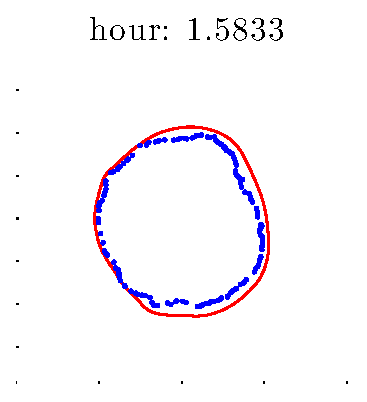
\includegraphics[height=.15\textheight]{Pos0/full/full2.eps}
		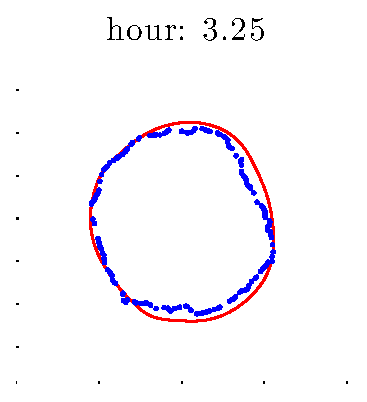
\includegraphics[height=.15\textheight]{Pos0/full/full3.eps}
		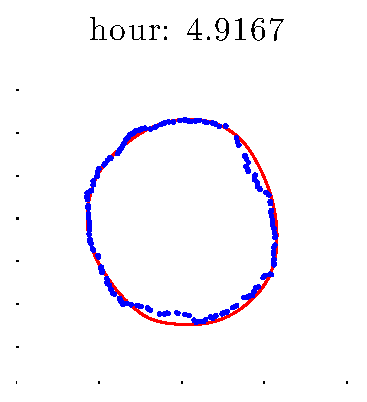
\includegraphics[height=.15\textheight]{Pos0/full/full4.eps}
		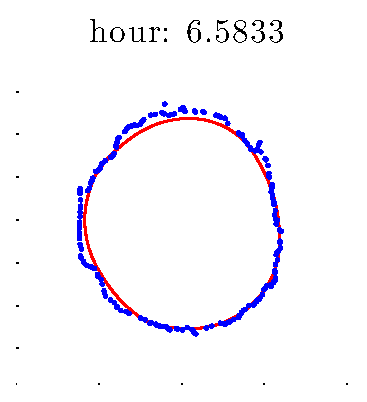
\includegraphics[height=.15\textheight]{Pos0/full/full5.eps}
		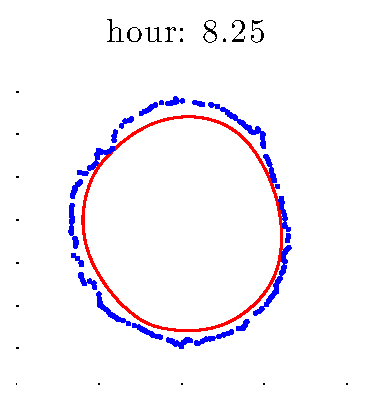
\includegraphics[height=.15\textheight]{Pos0/full/full6.eps}
		\caption{\textbf{Full} parameters: \\error 4188997.12169454}
	\end{subfigure}
	\begin{subfigure}[b]{.3\textwidth}
	\centering
		\includegraphics[height=.15\textheight]{Pos0/full/first1.eps}
		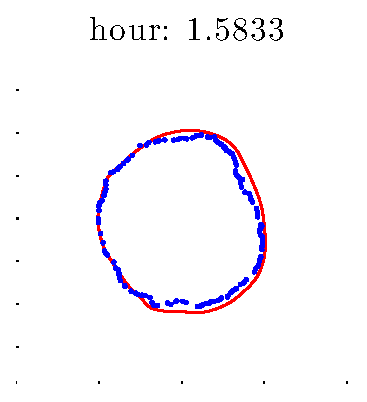
\includegraphics[height=.15\textheight]{Pos0/full/first2.eps}
		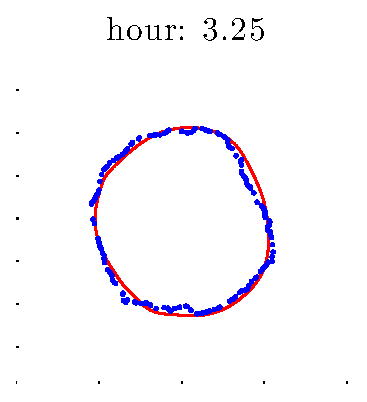
\includegraphics[height=.15\textheight]{Pos0/full/first3.eps}
		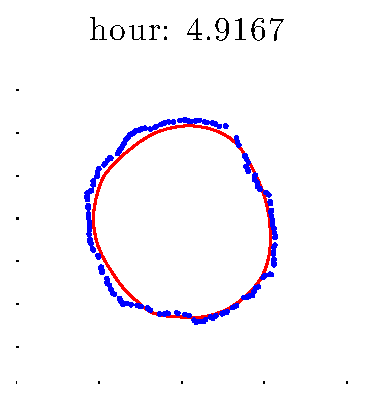
\includegraphics[height=.15\textheight]{Pos0/full/first4.eps}
		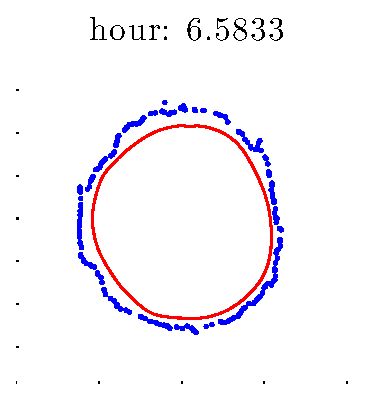
\includegraphics[height=.15\textheight]{Pos0/full/first5.eps}
		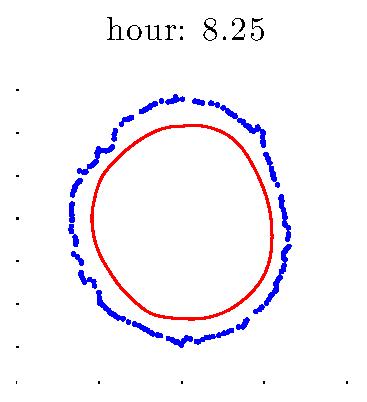
\includegraphics[height=.15\textheight]{Pos0/full/first6.eps}
		\caption{\textbf{First Half} parameters: \\error 4385995.22528114}
	\end{subfigure}
	\begin{subfigure}[b]{.3\textwidth}
	\centering
		\includegraphics[height=.15\textheight]{Pos0/full/second1.eps}
		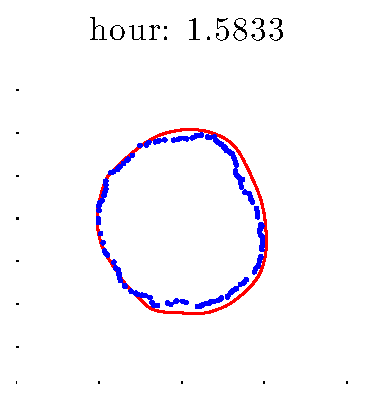
\includegraphics[height=.15\textheight]{Pos0/full/second2.eps}
		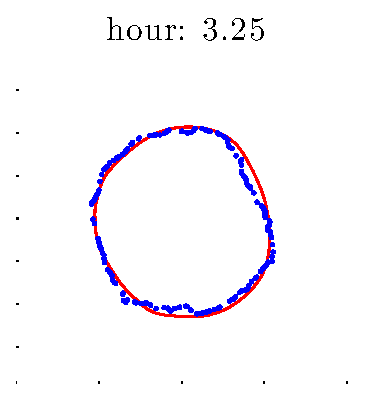
\includegraphics[height=.15\textheight]{Pos0/full/second3.eps}
		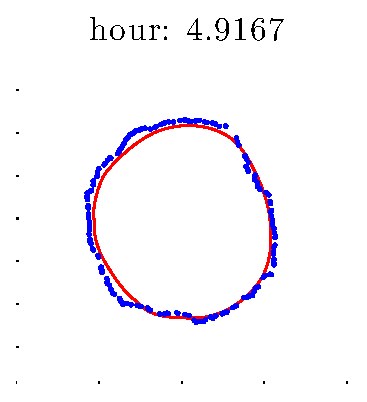
\includegraphics[height=.15\textheight]{Pos0/full/second4.eps}
		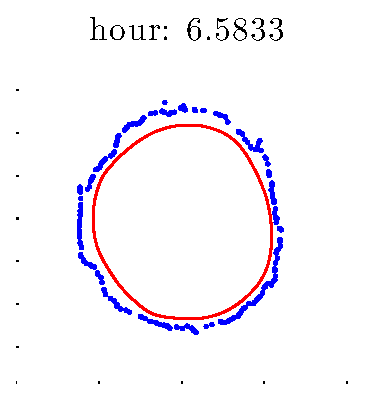
\includegraphics[height=.15\textheight]{Pos0/full/second5.eps}
		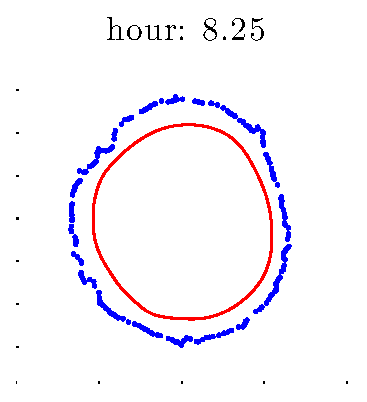
\includegraphics[height=.15\textheight]{Pos0/full/second6.eps}
		\caption{\textbf{Second Half} parameters: \\error 4393693.52587609}
	\end{subfigure}
\end{figure}

\clearpage

\noindent \textcolor{DarkGreen}{\textbf{Pos0:} Simulating the \textbf{First Half} time length (frames 1-60)}

\begin{figure}[h!]
\centering
	\begin{subfigure}[b]{.3\textwidth}
	\centering
		\includegraphics[height=.15\textheight]{Pos0/firsthalf/full1.eps}
		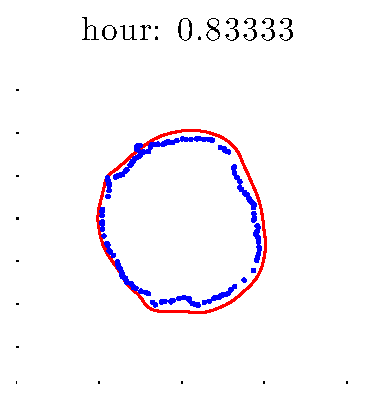
\includegraphics[height=.15\textheight]{Pos0/firsthalf/full2.eps}
		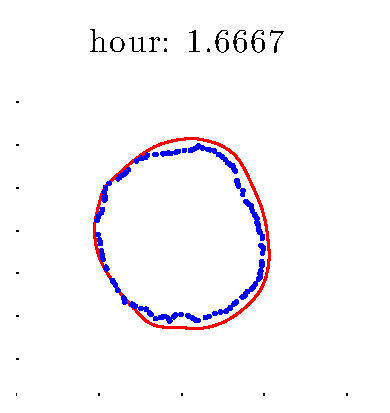
\includegraphics[height=.15\textheight]{Pos0/firsthalf/full3.eps}
		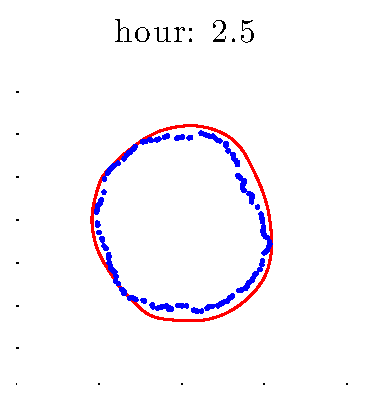
\includegraphics[height=.15\textheight]{Pos0/firsthalf/full4.eps}
		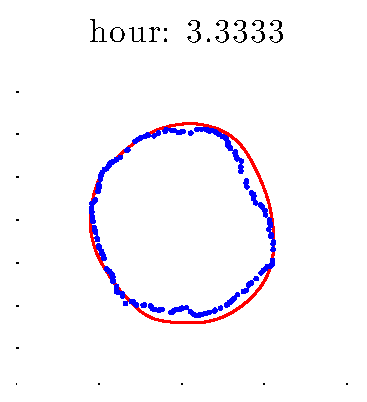
\includegraphics[height=.15\textheight]{Pos0/firsthalf/full5.eps}
		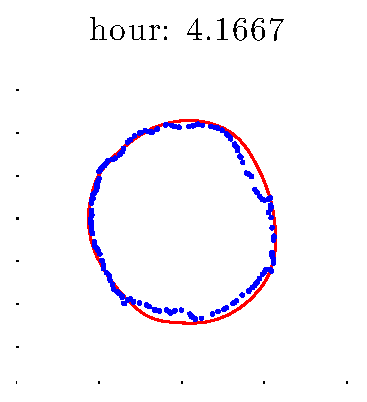
\includegraphics[height=.15\textheight]{Pos0/firsthalf/full6.eps}
		\caption{\textbf{Full} parameters: \\error 1324725.47344136}
	\end{subfigure}
	\begin{subfigure}[b]{.3\textwidth}
	\centering
		\includegraphics[height=.15\textheight]{Pos0/firsthalf/first1.eps}
		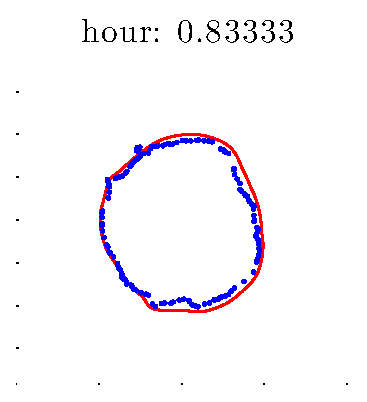
\includegraphics[height=.15\textheight]{Pos0/firsthalf/first2.eps}
		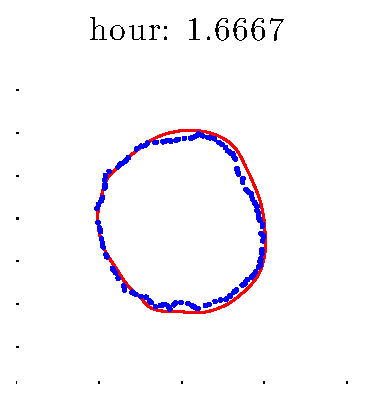
\includegraphics[height=.15\textheight]{Pos0/firsthalf/first3.eps}
		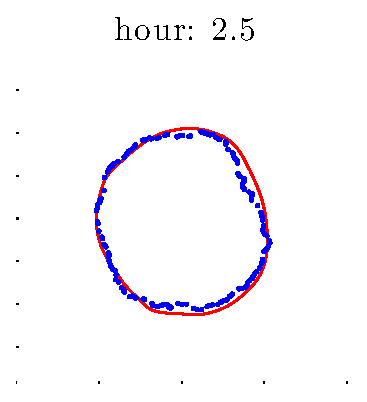
\includegraphics[height=.15\textheight]{Pos0/firsthalf/first4.eps}
		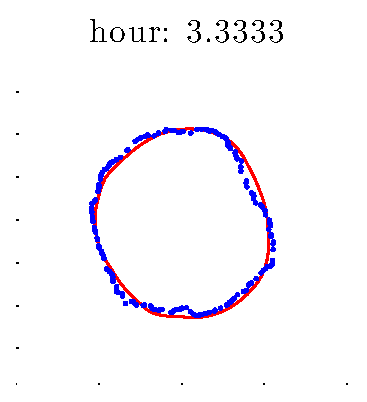
\includegraphics[height=.15\textheight]{Pos0/firsthalf/first5.eps}
		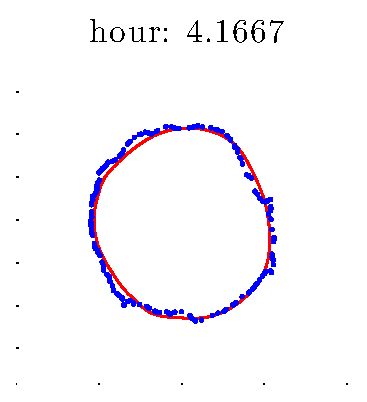
\includegraphics[height=.15\textheight]{Pos0/firsthalf/first6.eps}
		\caption{\textbf{First Half} parameters: \\error 1230368.12968762}
	\end{subfigure}
	\begin{subfigure}[b]{.3\textwidth}
	\centering
		\includegraphics[height=.15\textheight]{Pos0/firsthalf/second1.eps}
		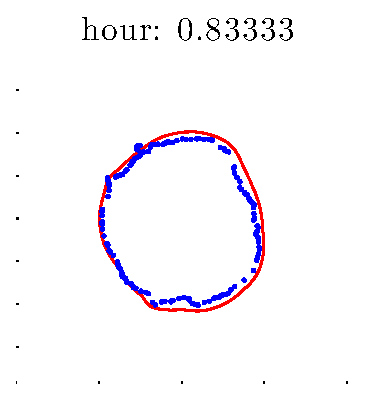
\includegraphics[height=.15\textheight]{Pos0/firsthalf/second2.eps}
		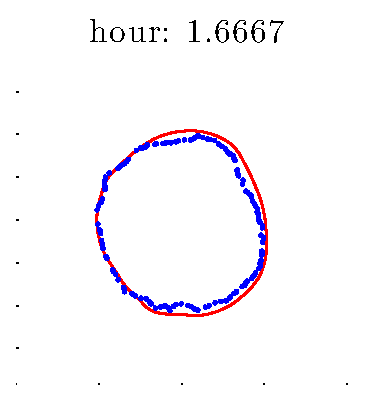
\includegraphics[height=.15\textheight]{Pos0/firsthalf/second3.eps}
		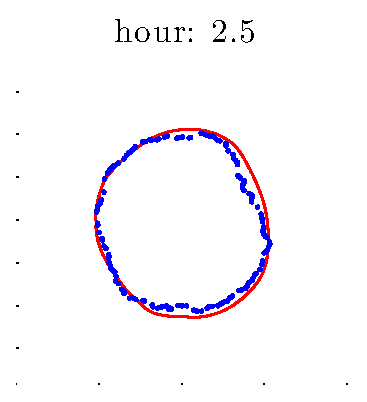
\includegraphics[height=.15\textheight]{Pos0/firsthalf/second4.eps}
		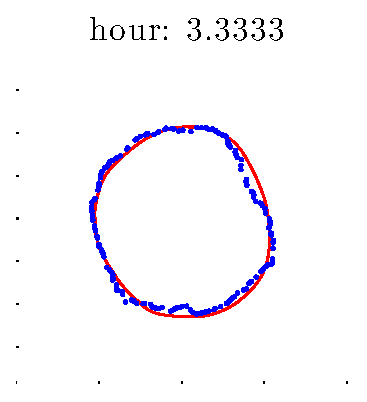
\includegraphics[height=.15\textheight]{Pos0/firsthalf/second5.eps}
		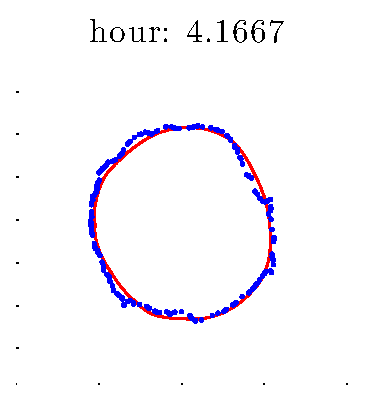
\includegraphics[height=.15\textheight]{Pos0/firsthalf/second6.eps}
		\caption{\textbf{Second Half} parameters: \\error 1243092.11017805}
	\end{subfigure}
\end{figure}

\clearpage

\noindent \textcolor{DarkGreen}{\textbf{Pos0:} Simulating the \textbf{Second Half} time length (frames 61-120) [\textit{hour 0 should be hour 5}]}

\begin{figure}[h!]
\centering
	\begin{subfigure}[b]{.3\textwidth}
	\centering
		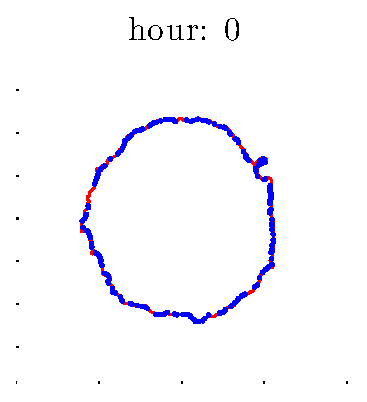
\includegraphics[height=.15\textheight]{Pos0/secondhalf/full1.eps}
		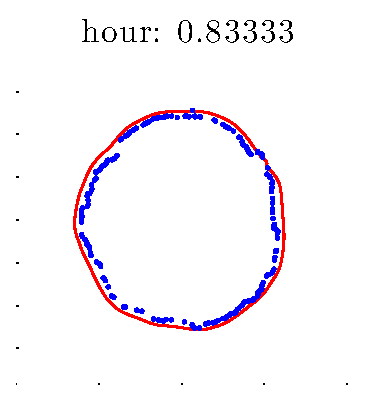
\includegraphics[height=.15\textheight]{Pos0/secondhalf/full2.eps}
		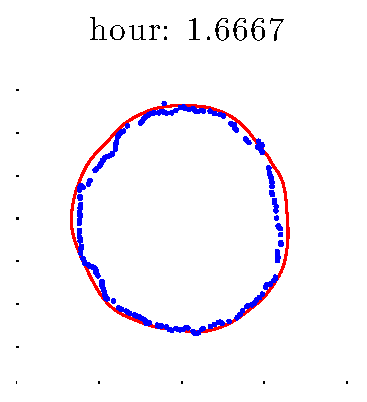
\includegraphics[height=.15\textheight]{Pos0/secondhalf/full3.eps}
		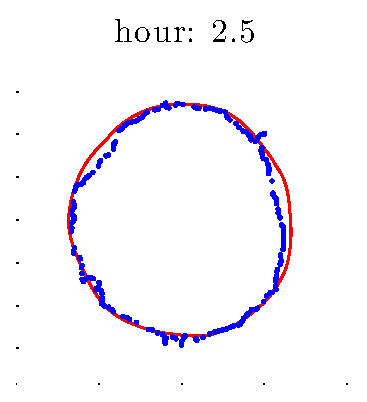
\includegraphics[height=.15\textheight]{Pos0/secondhalf/full4.eps}
		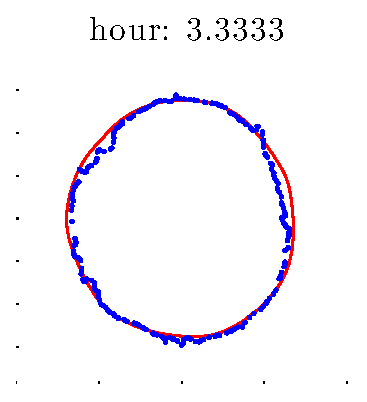
\includegraphics[height=.15\textheight]{Pos0/secondhalf/full5.eps}
		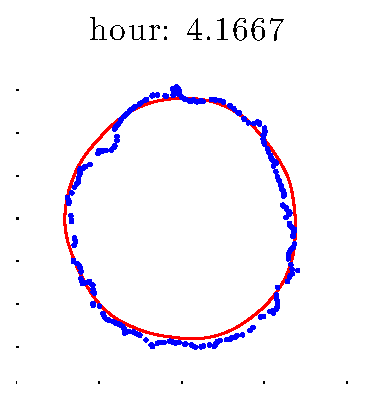
\includegraphics[height=.15\textheight]{Pos0/secondhalf/full6.eps}
		\caption{\textbf{Full} parameters: \\error 1590752.25980375}
	\end{subfigure}
	\begin{subfigure}[b]{.3\textwidth}
	\centering
		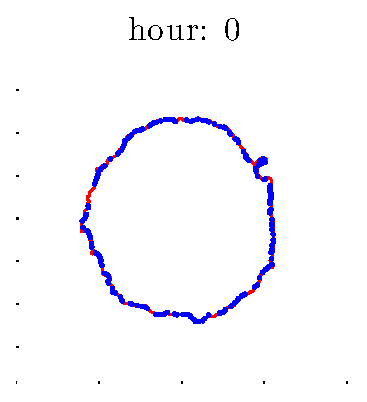
\includegraphics[height=.15\textheight]{Pos0/secondhalf/first1.eps}
		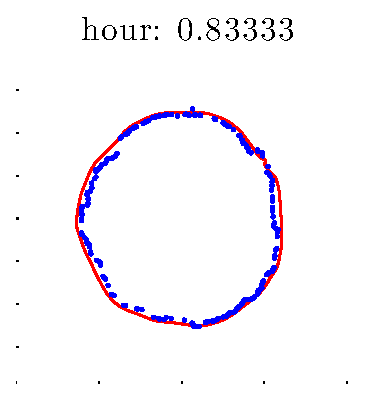
\includegraphics[height=.15\textheight]{Pos0/secondhalf/first2.eps}
		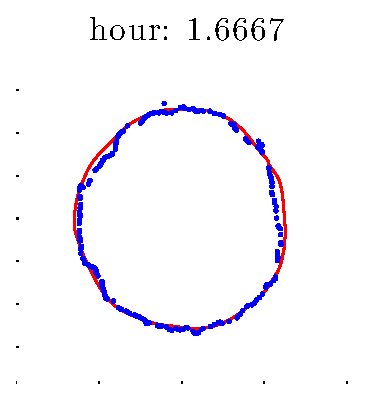
\includegraphics[height=.15\textheight]{Pos0/secondhalf/first3.eps}
		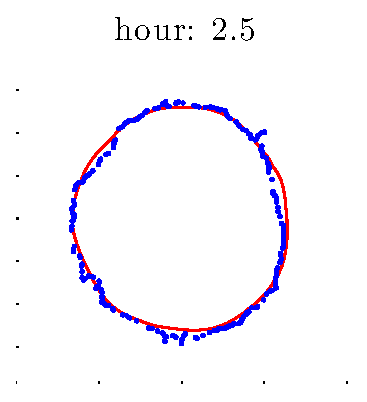
\includegraphics[height=.15\textheight]{Pos0/secondhalf/first4.eps}
		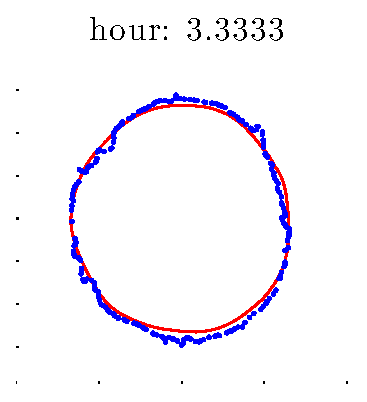
\includegraphics[height=.15\textheight]{Pos0/secondhalf/first5.eps}
		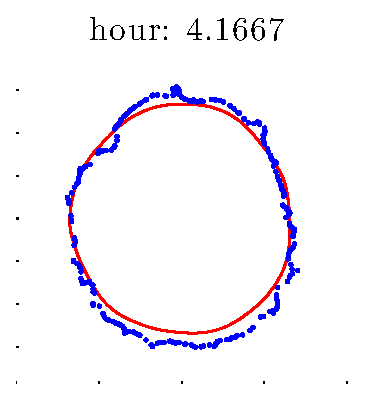
\includegraphics[height=.15\textheight]{Pos0/secondhalf/first6.eps}
		\caption{\textbf{First Half} parameters: \\error 1529213.46464141}
	\end{subfigure}
	\begin{subfigure}[b]{.3\textwidth}
	\centering
		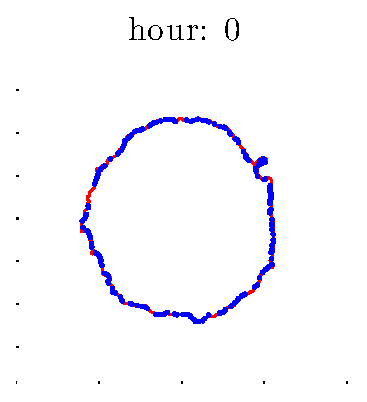
\includegraphics[height=.15\textheight]{Pos0/secondhalf/second1.eps}
		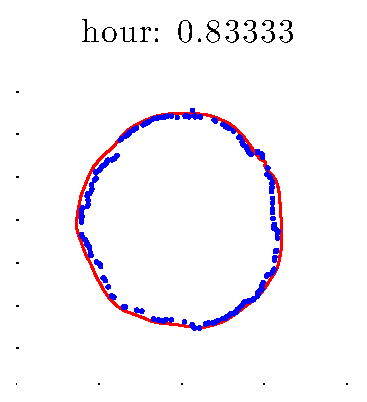
\includegraphics[height=.15\textheight]{Pos0/secondhalf/second2.eps}
		\includegraphics[height=.15\textheight]{Pos0/secondhalf/second3.eps}
		\includegraphics[height=.15\textheight]{Pos0/secondhalf/second4.eps}
		\includegraphics[height=.15\textheight]{Pos0/secondhalf/second5.eps}
		\includegraphics[height=.15\textheight]{Pos0/secondhalf/second6.eps}
		\caption{\textbf{Second Half} parameters: \\error 1428595.55645507}
	\end{subfigure}
\end{figure}























\vspace*{1in}
{\LARGE \textbf{Pos5 exp2}}
\vspace{.5in}
\begin{table}[h!]
    \begin{center}
    \Large
	\renewcommand{\arraystretch}{1.3}
        \begin{tabular}{|c|c|c|c|c|}
            \hline
		\textbf{Time Length} & \textbf{Estimated} $\boldsymbol F/\boldsymbol k$ & \textbf{Estimated} $\boldsymbol k/\boldsymbol b$ \\ \hline
		Full & 0.8012991691 & 6833.3317566531 \\ \hline
		First Half & 0.5242310598 & 10977.7104692166 \\ \hline
		Second Half & 0.5015108053 & 17038.3892808501 \\ \hline
        \end{tabular}
     \end{center}
\end{table}

\clearpage

\noindent \textcolor{DarkGreen}{\textbf{Pos5 exp2:} Simulating the \textbf{Full} time length (frames 1-120)}

\begin{figure}[h!]
\centering
	\begin{subfigure}[b]{.3\textwidth}
	\centering
		\includegraphics[height=.15\textheight]{Pos5exp2/full/full1.eps}
		\includegraphics[height=.15\textheight]{Pos5exp2/full/full2.eps}
		\includegraphics[height=.15\textheight]{Pos5exp2/full/full3.eps}
		\includegraphics[height=.15\textheight]{Pos5exp2/full/full4.eps}
		\includegraphics[height=.15\textheight]{Pos5exp2/full/full5.eps}
		\includegraphics[height=.15\textheight]{Pos5exp2/full/full6.eps}
		\caption{\textbf{Full} parameters: \\error 3468348.23811190}
	\end{subfigure}
	\begin{subfigure}[b]{.3\textwidth}
	\centering
		\includegraphics[height=.15\textheight]{Pos5exp2/full/first1.eps}
		\includegraphics[height=.15\textheight]{Pos5exp2/full/first2.eps}
		\includegraphics[height=.15\textheight]{Pos5exp2/full/first3.eps}
		\includegraphics[height=.15\textheight]{Pos5exp2/full/first4.eps}
		\includegraphics[height=.15\textheight]{Pos5exp2/full/first5.eps}
		\includegraphics[height=.15\textheight]{Pos5exp2/full/first6.eps}
		\caption{\textbf{First Half} parameters: \\error 3538670.56263672}
	\end{subfigure}
	\begin{subfigure}[b]{.3\textwidth}
	\centering
		\includegraphics[height=.15\textheight]{Pos5exp2/full/second1.eps}
		\includegraphics[height=.15\textheight]{Pos5exp2/full/second2.eps}
		\includegraphics[height=.15\textheight]{Pos5exp2/full/second3.eps}
		\includegraphics[height=.15\textheight]{Pos5exp2/full/second4.eps}
		\includegraphics[height=.15\textheight]{Pos5exp2/full/second5.eps}
		\includegraphics[height=.15\textheight]{Pos5exp2/full/second6.eps}
		\caption{\textbf{Second Half} parameters: \\error 3551127.88455402}
	\end{subfigure}
\end{figure}

\clearpage

\noindent \textcolor{DarkGreen}{\textbf{Pos5 exp2:} Simulating the \textbf{First Half} time length (frames 1-60)}

\begin{figure}[h!]
\centering
	\begin{subfigure}[b]{.3\textwidth}
	\centering
		\includegraphics[height=.15\textheight]{Pos5exp2/firsthalf/full1.eps}
		\includegraphics[height=.15\textheight]{Pos5exp2/firsthalf/full2.eps}
		\includegraphics[height=.15\textheight]{Pos5exp2/firsthalf/full3.eps}
		\includegraphics[height=.15\textheight]{Pos5exp2/firsthalf/full4.eps}
		\includegraphics[height=.15\textheight]{Pos5exp2/firsthalf/full5.eps}
		\includegraphics[height=.15\textheight]{Pos5exp2/firsthalf/full6.eps}
		\caption{\textbf{Full} parameters: \\error 1089865.32975761}
	\end{subfigure}
	\begin{subfigure}[b]{.3\textwidth}
	\centering
		\includegraphics[height=.15\textheight]{Pos5exp2/firsthalf/first1.eps}
		\includegraphics[height=.15\textheight]{Pos5exp2/firsthalf/first2.eps}
		\includegraphics[height=.15\textheight]{Pos5exp2/firsthalf/first3.eps}
		\includegraphics[height=.15\textheight]{Pos5exp2/firsthalf/first4.eps}
		\includegraphics[height=.15\textheight]{Pos5exp2/firsthalf/first5.eps}
		\includegraphics[height=.15\textheight]{Pos5exp2/firsthalf/first6.eps}
		\caption{\textbf{First Half} parameters: \\error 1048667.07794412}
	\end{subfigure}
	\begin{subfigure}[b]{.3\textwidth}
	\centering
		\includegraphics[height=.15\textheight]{Pos5exp2/firsthalf/second1.eps}
		\includegraphics[height=.15\textheight]{Pos5exp2/firsthalf/second2.eps}
		\includegraphics[height=.15\textheight]{Pos5exp2/firsthalf/second3.eps}
		\includegraphics[height=.15\textheight]{Pos5exp2/firsthalf/second4.eps}
		\includegraphics[height=.15\textheight]{Pos5exp2/firsthalf/second5.eps}
		\includegraphics[height=.15\textheight]{Pos5exp2/firsthalf/second6.eps}
		\caption{\textbf{Second Half} parameters: \\error 1059796.70390832}
	\end{subfigure}
\end{figure}

\clearpage

\noindent \textcolor{DarkGreen}{\textbf{Pos5 exp2:} Simulating the \textbf{Second Half} time length (frames 61-120) [\textit{hour 0 should be hour 5}]}

\begin{figure}[h!]
\centering
	\begin{subfigure}[b]{.3\textwidth}
	\centering
		\includegraphics[height=.15\textheight]{Pos5exp2/secondhalf/full1.eps}
		\includegraphics[height=.15\textheight]{Pos5exp2/secondhalf/full2.eps}
		\includegraphics[height=.15\textheight]{Pos5exp2/secondhalf/full3.eps}
		\includegraphics[height=.15\textheight]{Pos5exp2/secondhalf/full4.eps}
		\includegraphics[height=.15\textheight]{Pos5exp2/secondhalf/full5.eps}
		\includegraphics[height=.15\textheight]{Pos5exp2/secondhalf/full6.eps}
		\caption{\textbf{Full} parameters: \\error 1365164.56477798}
	\end{subfigure}
	\begin{subfigure}[b]{.3\textwidth}
	\centering
		\includegraphics[height=.15\textheight]{Pos5exp2/secondhalf/first1.eps}
		\includegraphics[height=.15\textheight]{Pos5exp2/secondhalf/first2.eps}
		\includegraphics[height=.15\textheight]{Pos5exp2/secondhalf/first3.eps}
		\includegraphics[height=.15\textheight]{Pos5exp2/secondhalf/first4.eps}
		\includegraphics[height=.15\textheight]{Pos5exp2/secondhalf/first5.eps}
		\includegraphics[height=.15\textheight]{Pos5exp2/secondhalf/first6.eps}
		\caption{\textbf{First Half} parameters: \\error 1343595.12364259}
	\end{subfigure}
	\begin{subfigure}[b]{.3\textwidth}
	\centering
		\includegraphics[height=.15\textheight]{Pos5exp2/secondhalf/second1.eps}
		\includegraphics[height=.15\textheight]{Pos5exp2/secondhalf/second2.eps}
		\includegraphics[height=.15\textheight]{Pos5exp2/secondhalf/second3.eps}
		\includegraphics[height=.15\textheight]{Pos5exp2/secondhalf/second4.eps}
		\includegraphics[height=.15\textheight]{Pos5exp2/secondhalf/second5.eps}
		\includegraphics[height=.15\textheight]{Pos5exp2/secondhalf/second6.eps}
		\caption{\textbf{Second Half} parameters: \\error 1326935.43227224}
	\end{subfigure}
\end{figure}























\vspace*{1in}
{\LARGE \textbf{Pos10 exp2}}
\vspace{.5in}
\begin{table}[h!]
    \begin{center}
    \Large
	\renewcommand{\arraystretch}{1.3}
        \begin{tabular}{|c|c|c|c|c|}
            \hline
		\textbf{Time Length} & \textbf{Estimated} $\boldsymbol F/\boldsymbol k$ & \textbf{Estimated} $\boldsymbol k/\boldsymbol b$ \\ \hline
		Full & 0.8314484349 & 3741.9517580108 \\ \hline
		First Half & 0.4371292942 & 5857.3294835273 \\ \hline
		Second Half & 0.570735699 & 12002.0206171335 \\ \hline
        \end{tabular}
     \end{center}
\end{table}

\clearpage

\noindent \textcolor{DarkGreen}{\textbf{Pos10 exp2:} Simulating the \textbf{Full} time length (frames 1-120)}

\begin{figure}[h!]
\centering
	\begin{subfigure}[b]{.3\textwidth}
	\centering
		\includegraphics[height=.15\textheight]{Pos10exp2/full/full1.eps}
		\includegraphics[height=.15\textheight]{Pos10exp2/full/full2.eps}
		\includegraphics[height=.15\textheight]{Pos10exp2/full/full3.eps}
		\includegraphics[height=.15\textheight]{Pos10exp2/full/full4.eps}
		\includegraphics[height=.15\textheight]{Pos10exp2/full/full5.eps}
		\includegraphics[height=.15\textheight]{Pos10exp2/full/full6.eps}
		\caption{\textbf{Full} parameters: \\error 4097361.38256544}
	\end{subfigure}
	\begin{subfigure}[b]{.3\textwidth}
	\centering
		\includegraphics[height=.15\textheight]{Pos10exp2/full/first1.eps}
		\includegraphics[height=.15\textheight]{Pos10exp2/full/first2.eps}
		\includegraphics[height=.15\textheight]{Pos10exp2/full/first3.eps}
		\includegraphics[height=.15\textheight]{Pos10exp2/full/first4.eps}
		\includegraphics[height=.15\textheight]{Pos10exp2/full/first5.eps}
		\includegraphics[height=.15\textheight]{Pos10exp2/full/first6.eps}
		\caption{\textbf{First Half} parameters: \\error 4223860.22175920}
	\end{subfigure}
	\begin{subfigure}[b]{.3\textwidth}
	\centering
		\includegraphics[height=.15\textheight]{Pos10exp2/full/second1.eps}
		\includegraphics[height=.15\textheight]{Pos10exp2/full/second2.eps}
		\includegraphics[height=.15\textheight]{Pos10exp2/full/second3.eps}
		\includegraphics[height=.15\textheight]{Pos10exp2/full/second4.eps}
		\includegraphics[height=.15\textheight]{Pos10exp2/full/second5.eps}
		\includegraphics[height=.15\textheight]{Pos10exp2/full/second6.eps}
		\caption{\textbf{Second Half} parameters: \\error 4205345.95231079}
	\end{subfigure}
\end{figure}

\clearpage

\noindent \textcolor{DarkGreen}{\textbf{Pos10 exp2:} Simulating the \textbf{First Half} time length (frames 1-60)}

\begin{figure}[h!]
\centering
	\begin{subfigure}[b]{.3\textwidth}
	\centering
		\includegraphics[height=.15\textheight]{Pos10exp2/firsthalf/full1.eps}
		\includegraphics[height=.15\textheight]{Pos10exp2/firsthalf/full2.eps}
		\includegraphics[height=.15\textheight]{Pos10exp2/firsthalf/full3.eps}
		\includegraphics[height=.15\textheight]{Pos10exp2/firsthalf/full4.eps}
		\includegraphics[height=.15\textheight]{Pos10exp2/firsthalf/full5.eps}
		\includegraphics[height=.15\textheight]{Pos10exp2/firsthalf/full6.eps}
		\caption{\textbf{Full} parameters: \\error 1136685.17157272}
	\end{subfigure}
	\begin{subfigure}[b]{.3\textwidth}
	\centering
		\includegraphics[height=.15\textheight]{Pos10exp2/firsthalf/first1.eps}
		\includegraphics[height=.15\textheight]{Pos10exp2/firsthalf/first2.eps}
		\includegraphics[height=.15\textheight]{Pos10exp2/firsthalf/first3.eps}
		\includegraphics[height=.15\textheight]{Pos10exp2/firsthalf/first4.eps}
		\includegraphics[height=.15\textheight]{Pos10exp2/firsthalf/first5.eps}
		\includegraphics[height=.15\textheight]{Pos10exp2/firsthalf/first6.eps}
		\caption{\textbf{First Half} parameters: \\error 1053128.48687592}
	\end{subfigure}
	\begin{subfigure}[b]{.3\textwidth}
	\centering
		\includegraphics[height=.15\textheight]{Pos10exp2/firsthalf/second1.eps}
		\includegraphics[height=.15\textheight]{Pos10exp2/firsthalf/second2.eps}
		\includegraphics[height=.15\textheight]{Pos10exp2/firsthalf/second3.eps}
		\includegraphics[height=.15\textheight]{Pos10exp2/firsthalf/second4.eps}
		\includegraphics[height=.15\textheight]{Pos10exp2/firsthalf/second5.eps}
		\includegraphics[height=.15\textheight]{Pos10exp2/firsthalf/second6.eps}
		\caption{\textbf{Second Half} parameters: \\error 1188303.05722478}
	\end{subfigure}
\end{figure}

\clearpage

\noindent \textcolor{DarkGreen}{\textbf{Pos10 exp2:} Simulating the \textbf{Second Half} time length (frames 61-120) [\textit{hour 0 should be hour 5}]}

\begin{figure}[h!]
\centering
	\begin{subfigure}[b]{.3\textwidth}
	\centering
		\includegraphics[height=.15\textheight]{Pos10exp2/secondhalf/full1.eps}
		\includegraphics[height=.15\textheight]{Pos10exp2/secondhalf/full2.eps}
		\includegraphics[height=.15\textheight]{Pos10exp2/secondhalf/full3.eps}
		\includegraphics[height=.15\textheight]{Pos10exp2/secondhalf/full4.eps}
		\includegraphics[height=.15\textheight]{Pos10exp2/secondhalf/full5.eps}
		\includegraphics[height=.15\textheight]{Pos10exp2/secondhalf/full6.eps}
		\caption{\textbf{Full} parameters: \\error 1736985.78216639}
	\end{subfigure}
	\begin{subfigure}[b]{.3\textwidth}
	\centering
		\includegraphics[height=.15\textheight]{Pos10exp2/secondhalf/first1.eps}
		\includegraphics[height=.15\textheight]{Pos10exp2/secondhalf/first2.eps}
		\includegraphics[height=.15\textheight]{Pos10exp2/secondhalf/first3.eps}
		\includegraphics[height=.15\textheight]{Pos10exp2/secondhalf/first4.eps}
		\includegraphics[height=.15\textheight]{Pos10exp2/secondhalf/first5.eps}
		\includegraphics[height=.15\textheight]{Pos10exp2/secondhalf/first6.eps}
		\caption{\textbf{First Half} parameters: \\error 1825332.39442093}
	\end{subfigure}
	\begin{subfigure}[b]{.3\textwidth}
	\centering
		\includegraphics[height=.15\textheight]{Pos10exp2/secondhalf/second1.eps}
		\includegraphics[height=.15\textheight]{Pos10exp2/secondhalf/second2.eps}
		\includegraphics[height=.15\textheight]{Pos10exp2/secondhalf/second3.eps}
		\includegraphics[height=.15\textheight]{Pos10exp2/secondhalf/second4.eps}
		\includegraphics[height=.15\textheight]{Pos10exp2/secondhalf/second5.eps}
		\includegraphics[height=.15\textheight]{Pos10exp2/secondhalf/second6.eps}
		\caption{\textbf{Second Half} parameters: \\error 1551458.41010493}
	\end{subfigure}
\end{figure}























\vspace*{1in}
{\LARGE \textbf{Pos14 exp8}}
\vspace{.5in}
\begin{table}[h!]
    \begin{center}
    \Large
	\renewcommand{\arraystretch}{1.3}
        \begin{tabular}{|c|c|c|c|c|}
            \hline
		\textbf{Time Length} & \textbf{Estimated} $\boldsymbol F/\boldsymbol k$ & \textbf{Estimated} $\boldsymbol k/\boldsymbol b$ \\ \hline
		Full & 1.0711682858 & 2832.2499810798 \\ \hline
		First Half & 0.7395095223 & 4622.6470044375 \\ \hline
		Second Half & 0.578052328 & 6794.1595948324 \\ \hline
        \end{tabular}
     \end{center}
\end{table}

\clearpage

\noindent \textcolor{DarkGreen}{\textbf{Pos14 exp8:} Simulating the \textbf{Full} time length (frames 1-120)}

\begin{figure}[h!]
\centering
	\begin{subfigure}[b]{.3\textwidth}
	\centering
		\includegraphics[height=.15\textheight]{Pos14exp8/full/full1.eps}
		\includegraphics[height=.15\textheight]{Pos14exp8/full/full2.eps}
		\includegraphics[height=.15\textheight]{Pos14exp8/full/full3.eps}
		\includegraphics[height=.15\textheight]{Pos14exp8/full/full4.eps}
		\includegraphics[height=.15\textheight]{Pos14exp8/full/full5.eps}
		\includegraphics[height=.15\textheight]{Pos14exp8/full/full6.eps}
		\caption{\textbf{Full} parameters: \\error 4053533.70424384}
	\end{subfigure}
	\begin{subfigure}[b]{.3\textwidth}
	\centering
		\includegraphics[height=.15\textheight]{Pos14exp8/full/first1.eps}
		\includegraphics[height=.15\textheight]{Pos14exp8/full/first2.eps}
		\includegraphics[height=.15\textheight]{Pos14exp8/full/first3.eps}
		\includegraphics[height=.15\textheight]{Pos14exp8/full/first4.eps}
		\includegraphics[height=.15\textheight]{Pos14exp8/full/first5.eps}
		\includegraphics[height=.15\textheight]{Pos14exp8/full/first6.eps}
		\caption{\textbf{First Half} parameters: \\error 4085190.10957947}
	\end{subfigure}
	\begin{subfigure}[b]{.3\textwidth}
	\centering
		\includegraphics[height=.15\textheight]{Pos14exp8/full/second1.eps}
		\includegraphics[height=.15\textheight]{Pos14exp8/full/second2.eps}
		\includegraphics[height=.15\textheight]{Pos14exp8/full/second3.eps}
		\includegraphics[height=.15\textheight]{Pos14exp8/full/second4.eps}
		\includegraphics[height=.15\textheight]{Pos14exp8/full/second5.eps}
		\includegraphics[height=.15\textheight]{Pos14exp8/full/second6.eps}
		\caption{\textbf{Second Half} parameters: \\error 4145230.23342968}
	\end{subfigure}
\end{figure}

\clearpage

\noindent \textcolor{DarkGreen}{\textbf{Pos14 exp8:} Simulating the \textbf{First Half} time length (frames 1-60)}

\begin{figure}[h!]
\centering
	\begin{subfigure}[b]{.3\textwidth}
	\centering
		\includegraphics[height=.15\textheight]{Pos14exp8/firsthalf/full1.eps}
		\includegraphics[height=.15\textheight]{Pos14exp8/firsthalf/full2.eps}
		\includegraphics[height=.15\textheight]{Pos14exp8/firsthalf/full3.eps}
		\includegraphics[height=.15\textheight]{Pos14exp8/firsthalf/full4.eps}
		\includegraphics[height=.15\textheight]{Pos14exp8/firsthalf/full5.eps}
		\includegraphics[height=.15\textheight]{Pos14exp8/firsthalf/full6.eps}
		\caption{\textbf{Full} parameters: \\error 1313678.93217561}
	\end{subfigure}
	\begin{subfigure}[b]{.3\textwidth}
	\centering
		\includegraphics[height=.15\textheight]{Pos14exp8/firsthalf/first1.eps}
		\includegraphics[height=.15\textheight]{Pos14exp8/firsthalf/first2.eps}
		\includegraphics[height=.15\textheight]{Pos14exp8/firsthalf/first3.eps}
		\includegraphics[height=.15\textheight]{Pos14exp8/firsthalf/first4.eps}
		\includegraphics[height=.15\textheight]{Pos14exp8/firsthalf/first5.eps}
		\includegraphics[height=.15\textheight]{Pos14exp8/firsthalf/first6.eps}
		\caption{\textbf{First Half} parameters: \\error 1302107.57869745}
	\end{subfigure}
	\begin{subfigure}[b]{.3\textwidth}
	\centering
		\includegraphics[height=.15\textheight]{Pos14exp8/firsthalf/second1.eps}
		\includegraphics[height=.15\textheight]{Pos14exp8/firsthalf/second2.eps}
		\includegraphics[height=.15\textheight]{Pos14exp8/firsthalf/second3.eps}
		\includegraphics[height=.15\textheight]{Pos14exp8/firsthalf/second4.eps}
		\includegraphics[height=.15\textheight]{Pos14exp8/firsthalf/second5.eps}
		\includegraphics[height=.15\textheight]{Pos14exp8/firsthalf/second6.eps}
		\caption{\textbf{Second Half} parameters: \\error 1311780.79305664}
	\end{subfigure}
\end{figure}

\clearpage

\noindent \textcolor{DarkGreen}{\textbf{Pos14 exp8:} Simulating the \textbf{Second Half} time length (frames 61-120) [\textit{hour 0 should be hour 5}]}

\begin{figure}[h!]
\centering
	\begin{subfigure}[b]{.3\textwidth}
	\centering
		\includegraphics[height=.15\textheight]{Pos14exp8/secondhalf/full1.eps}
		\includegraphics[height=.15\textheight]{Pos14exp8/secondhalf/full2.eps}
		\includegraphics[height=.15\textheight]{Pos14exp8/secondhalf/full3.eps}
		\includegraphics[height=.15\textheight]{Pos14exp8/secondhalf/full4.eps}
		\includegraphics[height=.15\textheight]{Pos14exp8/secondhalf/full5.eps}
		\includegraphics[height=.15\textheight]{Pos14exp8/secondhalf/full6.eps}
		\caption{\textbf{Full} parameters: \\error 1439465.35670884}
	\end{subfigure}
	\begin{subfigure}[b]{.3\textwidth}
	\centering
		\includegraphics[height=.15\textheight]{Pos14exp8/secondhalf/first1.eps}
		\includegraphics[height=.15\textheight]{Pos14exp8/secondhalf/first2.eps}
		\includegraphics[height=.15\textheight]{Pos14exp8/secondhalf/first3.eps}
		\includegraphics[height=.15\textheight]{Pos14exp8/secondhalf/first4.eps}
		\includegraphics[height=.15\textheight]{Pos14exp8/secondhalf/first5.eps}
		\includegraphics[height=.15\textheight]{Pos14exp8/secondhalf/first6.eps}
		\caption{\textbf{First Half} parameters: \\error 1404379.23730973}
	\end{subfigure}
	\begin{subfigure}[b]{.3\textwidth}
	\centering
		\includegraphics[height=.15\textheight]{Pos14exp8/secondhalf/second1.eps}
		\includegraphics[height=.15\textheight]{Pos14exp8/secondhalf/second2.eps}
		\includegraphics[height=.15\textheight]{Pos14exp8/secondhalf/second3.eps}
		\includegraphics[height=.15\textheight]{Pos14exp8/secondhalf/second4.eps}
		\includegraphics[height=.15\textheight]{Pos14exp8/secondhalf/second5.eps}
		\includegraphics[height=.15\textheight]{Pos14exp8/secondhalf/second6.eps}
		\caption{\textbf{Second Half} parameters: \\error 1394108.38474321}
	\end{subfigure}
\end{figure}




\end{document}